%%%%%%%%%%%%%%%%%%%%%%%%%%%%%
%%%%%%%%%%%%%%%%%%%%%%%%%%%%%

\chapter{Introduction: The Two Cultures of Behavioral Sciences}
\pagenumbering{arabic}
\setcounter{page}{1}


\begin{comment}
    

The motivation of what the problem is and why we need to solve the problem can come from social algorithms, marketing, and also LLMs, human alignment.

The motivation of how we need to solve the problem can come from shannon, LLM training, and two approaches of statistical learning.

<communicator, content/item/message, channel, time, receiver, effect/rating>
<content, effect> prediction and selecting content to optimize effect -> recommendation, CTR prediction
receiver optimization -> personalization

What we are proposing -> better CTR prediction especially in low data settings, effective content generation, better explanation, 



\end{comment}



Behavior as a modality\footnote{A \textit{modality} is defined in terms of information, such that a modality is a medium through which information is conveyed \cite{liang2022foundations,grifoni2009multimodal,martin2001annotation}. Similarly, a multimodal distribution is defined as having more than one peak in the probability distribution describing the nature of information.} occurs in the process of communication. Communication includes all of the procedures by which one mind may affect another \cite{shannon-weaver-1949}. This includes all forms of expression, such as words, gestures, speech, pictures, and musical sounds. Communication can be seen as being composed of seven modalities (Fig.~\ref{fig:factors-of-communication}): (the communicator, message, time of message (or time of receipt), channel, receiver, time of effect, and effect). These modalities can vary independently of each other \cite{khandelwal2023large,khurana-etal-2023-synthesizing,si2023long,khurana2023behavior} and carry signals about each other \cite{khurana-etal-2023-synthesizing,bhattacharya2023video}. The message as a modality carries information from the communicator to receiver and encodes information generated by the communicator. Similarly, behavior (\textit{aka} effect) as a modality carries information from the receiver and encodes information generated by the receiver. This is often a continuous cycle, where behavior generated in the previous cycle becomes the message of the next cycle, thus forming a (continuous) conversation. 



Different fields of behavioral sciences deal with different parts of behavior. we will give a broad overview of these fields in the upcoming paragraphs, but two streams have emerged broadly in behavioral sciences: explanation and prediction of behavior (receiver effect) \cite{breiman2001statistical,hofman2017prediction,shmueli2010explain}. 


\begin{figure*}[!t]
  \centering
  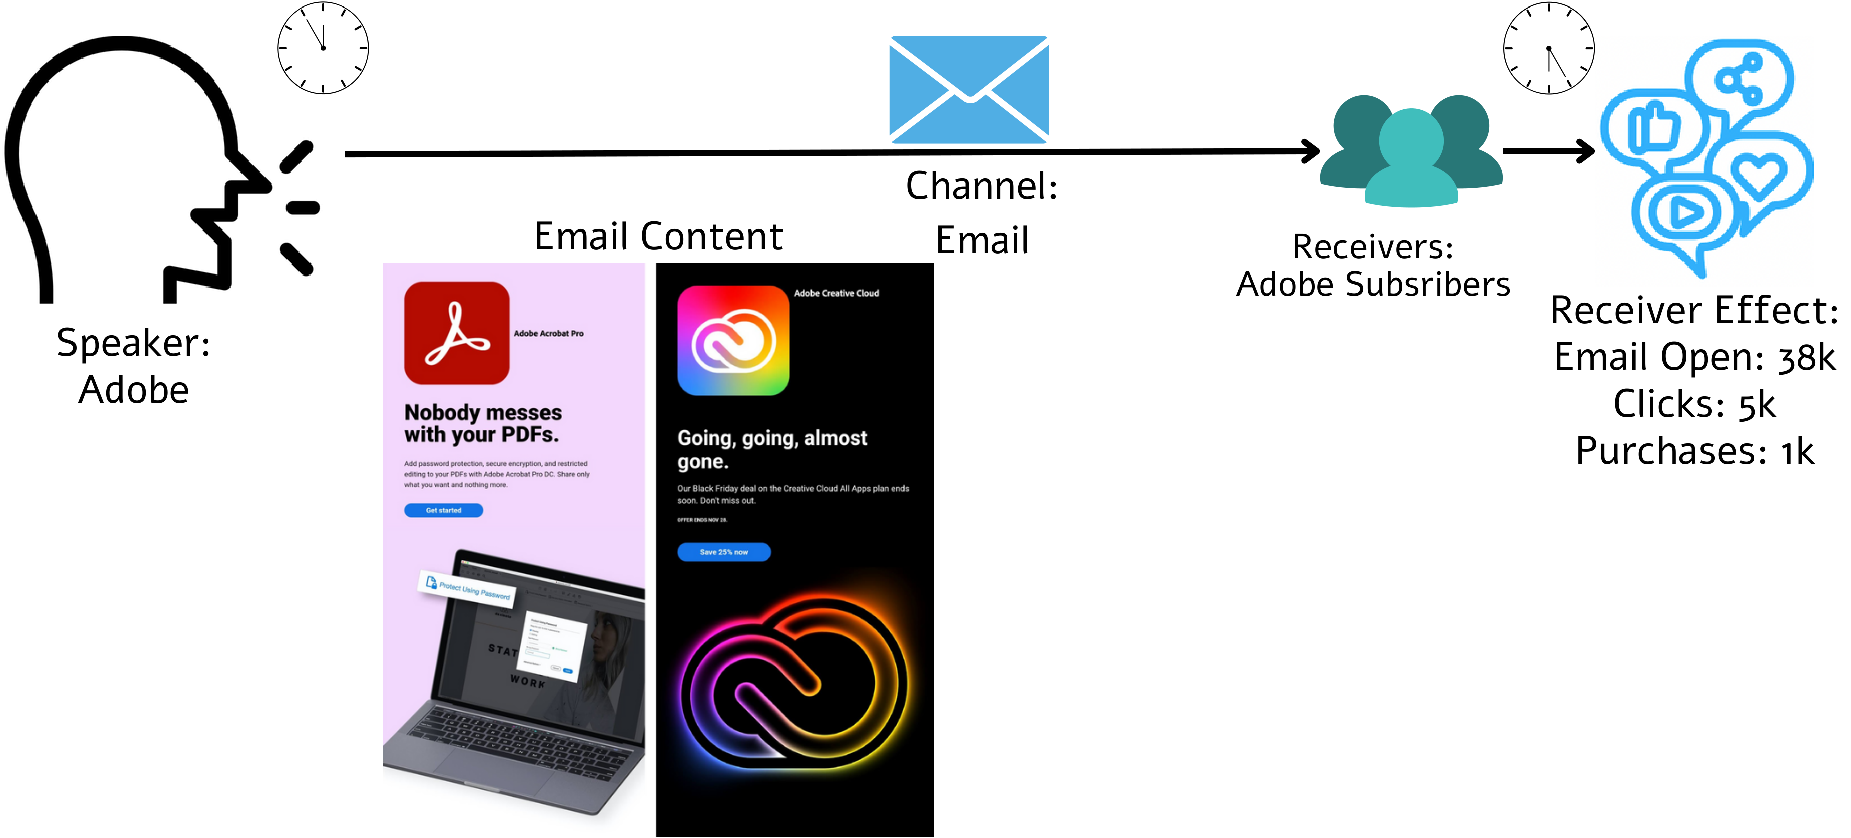
\includegraphics[width=1.0\textwidth]{images/factors of communication.pdf}
  \caption{Communication process can be defined by seven factors: Communicator, Message, Time of message, Channel, Receiver, Time of effect, and Effect. Any message is created to serve an end goal. For marketers, the end goal is to bring in the desired receiver effect (behavior) (like clicks, purchases, likes, and customer retention). The figure presents the key elements in the communication pipeline - the marketer, message, channel, receivers, and finally, the receiver effect.   \label{fig:factors-of-communication}}
\end{figure*}

Historically, behavioral social scientists have sought explanations of human behavior that can provide interpretable causal mechanisms behind human functioning. A few prominent examples are Milgram's \cite{milgram1978obedience} and Asch's \cite{asch1948doctrine} experiments on persuasion, explaining the causal mechanism of obedience to authority. The approach of theorizing has worked in physical sciences where the data is plentiful, and theories make unambiguous predictions but have not been too successful in \textit{predicting} social outcomes in behavioral sciences \cite{open2015estimating,tetlock2017expert,forecasting2023insights}. In fact, many studies have shown that expert human opinions fare similar to non-experts (\textit{e.g.}, predicting economic and political trends \cite{tetlock2017expert}, societal change: \cite{forecasting2023insights}, and advertising success: \cite{singh2024measuring}), and the opinion of non-expert population is roughly the same as a random coin toss in predicting behavior (\textit{e.g.}, predicting cascades \cite{tan2014effect} or image memorability \cite{isola2013makes}). At the same time, causal mechanisms have their own merits; most notably, they help decision-makers (often humans) to make intuitive sense of the situation and make their next decision based on it. 


In parallel, due to the availability of human behavior data at scale, researchers in machine learning are showing a growing interest in traditionally behavioral science topics, such as messaging strategies leading to persuasion \cite{habernal2016makes,kumar2023persuasion,luu2019measuring,bhattacharya2023video}, information diffusion \cite{cheng2014can,martin2016exploring}, and most importantly, prediction and predictability of human behavior \cite{choi2012predicting,song2010limits}. Machine learning approaches bring with them the culture of (training and) testing their models on large real-world datasets and pushing the state-of-the-art in terms of predictive accuracies; at the same time, often, ML approaches can only be operated as black boxes with no direct mechanism to explain predictions \cite{salganik2019bit,singla2022audio}.



In the prediction community, different subfields have emerged dealing with the different parts of the problem of optimization of human behavior. For instance, advertisement personalization studies how to optimize (choose) \textit{receiver} for a given message \cite{chandra2022personalization}, and recommendation systems study how to \textit{choose content} from a set of pre-decided contents for a given receiver to elicit a certain effect \cite{herlocker2004evaluating}. A popular problem within the prediction community is the effect prediction problems, for example, clickthrough (CTR) prediction \cite{mcmahan2013ad}, Twitter cascade prediction \cite{cheng2014can,martin2016exploring}, sales prediction \cite{choi2012predicting,pryzant2017predicting}, content memorability prediction \cite{isola2011makes,khosla2015understanding,si2023long}, \textit{etc}. There are also works to optimize the time of the message to elicit certain effect \cite{newstead2010cost,si2023long}. Some of the major problems studied in behavioral sciences are given below. Through this list, one can observe that all the factors of communication are studied independently in their own light without relying on the underlying unity and continuity of the communication process. 


\begin{enumerate}
\item \textbf{Problems related to optimization in the sender space}:
    \begin{enumerate}
        \item \textbf{Source Optimization}: \textit{Who} should send a particular message over a channel to a specific audience to get the desired behavior? This includes selecting between different brand voices, influencers, spokespersons, or organizational entities based on authority, trustworthiness, and audience affinity.
    \end{enumerate}
    

\item Problems related to Receiver optimization:
    \begin{enumerate}
        \item \textbf{Personalization}: Identifying the optimal receiver for a specific content-channel-time combination to maximize engagement and conversion probability.
        \item \textbf{Customer Segmentation}: Strategic division of the customer base into distinct, actionable groups based on shared characteristics, behaviors, or value propositions to enable differentiated marketing approaches.
        \item \textbf{Social Network Analysis}: Modelling the interconnectedness of receivers (and senders) together in a graph to describe social phenomena like contagion and homophily.
        \item \textbf{Lookalike Modeling}:  Identifying and targeting prospective customers who share similar characteristics, behaviors, and propensities with existing high-value customers or target audiences.
        \item \textbf{Market surveys}: Systematic collection and analysis of primary data about target markets, customer preferences, and competitive landscape to inform marketing decisions.
        \item \textbf{Identity stitching}: Probabilistic and deterministic matching of cross-channel, cross-device customer actions to create unified customer profiles and journey maps.
        \item \textbf{Behavior Explanation}: Discovering causal mechanisms behind a receiver action.
    \end{enumerate}
    
\item \textbf{Problems related to optimization in the content space}:
    \begin{enumerate}
        \item \textbf{Recommender Systems}: Identifying the optimal content that should be delivered next to a certain receiver given a fixed channel, time, and a repository of contents (and their corresponding senders).
        \item \textbf{A/B Testing}: A randomized experiment involving two or more variants with the goal of discovering which variant of a message performs better with a certain audience.
        \item \textbf{Customer Targeting}: Determining what message should be delivered to a target audience segment, targeted based on multi-dimensional attributes (geographic, demographic, behavioral, and psychographic) through particular channels.

        \item \textbf{Propensity Modelling or Engagement Modelling}: Modeling probability of engagement in terms of actions like Clickthrough, social media actions such as likes and shares for a certain audience, sender, and campaign.
        \item \textbf{Transsuasion}: Conversion of a content from low-performing to high-performing for a given audience, sender, and time, while maintaining the content's intent, style, and emotional impact.
        \item \textbf{Transcreation}: Conversion of a content designed for one audience (like a particular culture) to another audience, while maintaining the content's intent, style, and emotional impact.
        \item \textbf{Search Engine Optimization}: Improving the quality and quantity of website traffic to a website from search engines by doing content optimization (like adding keywords, backlinks, \textit{etc}).
        \item \textbf{Performant Content Generation}: Generate content that can perform better for a given audience, sender, time, and goal.
        \item \textbf{Argument Mining}: Automatic extraction and identification of argumentative structures from natural language text.
        \item \textbf{Persuasion Strategies}: Use of rhetorical devices (such as emotion, social identity, and scarcity) to optimize the effect of a message on a certain audience.
    \end{enumerate}

\item \textbf{Problems related to optimization in the channel space}:
    \begin{enumerate}
        \item \textbf{Channel Optimization}: Optimizing channels for a particular audience, sender, time, and goal.
        \item \textbf{Marketing Mix Modeling}: Measuring and attributing the impact of various decisions like channel investments, discounts, promotional campaigns in their contribution to engagement and sales. 
        \item \textbf{Auction Design} and \textbf{Bidding}: Mechanisms to discover the cost of attention of a certain receiver to a particular sender, time, and campaign goal.
    \end{enumerate}
    
\item \textbf{Problem related to optimization in the time space}:
    \begin{enumerate}
        \item \textbf{Send Time Optimization}: Determining the optimal timing for message delivery for a certain receiver, sender, content combination.

        \item \textbf{Trend Forecasting}: Projecting marketing and social trends in the future.
    \end{enumerate}
        
\end{enumerate}







A common theme that runs through both research cultures in behavioral sciences is the intent to control behavior. Explanation and prediction are intermediate steps to control and hence optimize behavior. Optimizing behavior means to fulfill the communicator's objectives by controlling the other six parts of the communication process (Fig.~\ref{fig:factors-of-communication}). Due to the problem space being large, the solution needs a general understanding of human behavior as opposed to being domain-specific. In this thesis, our aim is to make such models that can develop this general understanding.


The characteristic that marks the digital age is the prevalence of human behavioral data in huge repositories. This data is \textit{big} (allowing to model heterogeneity), \textit{always-on} (allowing to look in the past as well as live measurements), observational (as opposed to reactive), but also \textit{incomplete} (does not capture all that is happening everywhere everytime in a single repository) and \textit{algorithmically confounded} (generated as a byproduct of an engineering process with a goal) \cite{salganik2019bit}. While the predictive culture has tried to make use of some of this data in the form of social media datasets like Twitter \cite{tumasjan2010predicting,asur2010predicting} and Instagram \cite{kim2020multimodal}, Google trends \cite{choi2012predicting,carriere2013nowcasting}, Wikipedia \cite{generous2014global,de2021general,mestyan2013early}, shopping websites \cite{krumme2013predictability,de2015unique} and other data sources \cite{brockmann2006scaling,song2010limits,miritello2013limited}, these efforts are limited, in the sense of being dependent on one or a few chosen platforms, able to answer a limited set of questions, and restricted by access to private data. We want a model that can understand (predict and explain) \textit{human behavior in general} as opposed to modeling a particular effect (retweet prediction) on a particular platform (\textit{e.g.} Twitter) for a certain type of users.
This problem carries parallels with the problem being solved in the natural language processing (NLP) community, where supervised models in NLP are limited by the amount of supervision available and being able to answer one question (for which the supervised model was trained). The problem was solved by developing Large Language Models (LLMs), which are general purpose models capable of \textit{understanding language}, and hence can solve natural language tasks like sentiment analysis, question answering, email generation, and language translation in zero-shot (\textit{i.e.} without needing any explicit training for that task) \cite{devlin2018bert,brown2020language,radford2018improving,raffel2020exploring,radford2019language}.





\begin{figure*}[h]
  \centering
  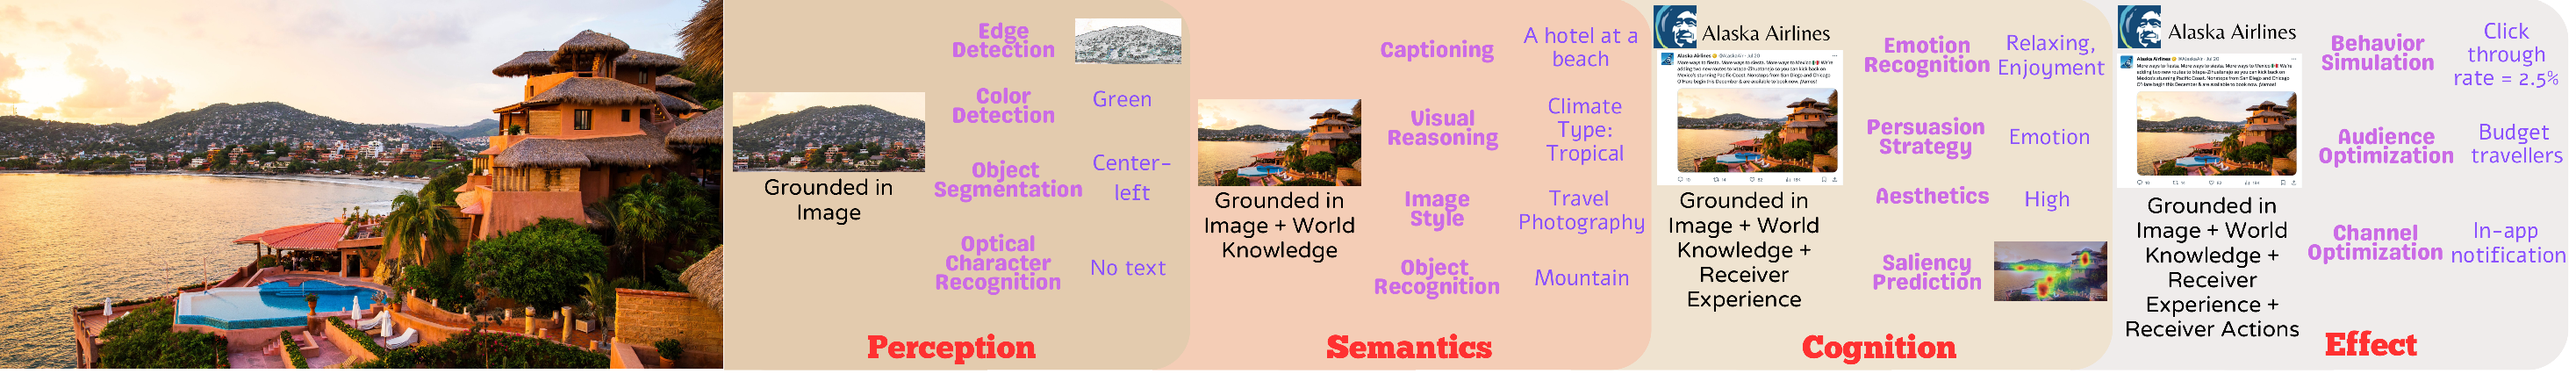
\includegraphics[width=1.0\textwidth]{images/levels of analysis.pdf}
  \caption{Levels of content analysis. The figure lists tasks and their sample outputs arranged in a hierarchy \cite{shannon-weaver-1949}. This is roughly based on levels of language. Notably, humans are good at predicting the first three levels but not the last level \cite{tetlock2017expert,forecasting2023insights,tan2014effect,isola2013makes}. 
  \label{fig:levels of content analysis}
  }
\end{figure*}


Similarly, how do we develop a model capable of understanding behavior \textit{in general}? With the intent to answer this question, we take motivation from LLMs, where the idea is to train a model on a data-rich task. The task chosen to train LLMs is the next-word prediction, and the dataset is the text collected from the entire internet. The next-word prediction task is a data-rich task that can be trained on the huge text repositories from the internet. The intuition is that two approaches have always worked for neural networks: larger model sizes and more data for training \cite{mikolov2013efficient,devlin2018bert,radford2018improving,raffel2020exploring}. Going from a few million tokens of text \cite{mikolov2013efficient,radford2018improving} to a trillion tokens \cite{touvron2023llama,brown2020language} leads to an increase in the transfer learning capability leading to performance improvements over a wide variety of natural language tasks. 


The digital revolution has provided us with huge repositories of data. We leverage the human behavior repositories available on the internet for this general-purpose human behavior model. The format of this data is the general communication model shown in Fig.~\ref{fig:factors-of-communication} consisting of communicator, message, time of message, channel, receiver, time of effect, and effect. Due to the incomplete nature of behavioral repositories, all the factors are usually not always available. However, a subset is always available, and we show that the data scale, along with a large model, helps make a general behavior understanding model \cite{khandelwal2023large}. We call this model, Large Content and Behavior Model (LCBM). We show that LCBM can predict behavior, explain it, and generate a message to bring about certain behavior \cite{si2023long,khandelwal2023large,khurana2023behavior}. 



\textit{Are general LLMs unable to solve behavioral problems?} A question that arises is whether LLMs, which already learn trillions of text tokens, are able to understand and predict behavior. We investigate that question over several large models, including GPT-3.5 \cite{brown2020language}, GPT-4 \cite{openai2023gpt4}, Llama-13 B and LLama-7B \cite{touvron2023llama}, and find that they are unable to solve the behavioral problems listed before. The reason for this is that large language models only include one factor (message) out of the 7-factor communication model (Fig.~\ref{fig:factors-of-communication}) while considering other parts as ``noise'' (for instance, see \cite{biderman2022datasheet,penedo2023refinedweb}). This systematic purge of communicator, receiver, channel, time, and, most importantly, behavior causes the models not to develop any behavioral capabilities (Level-C of Shannon and Weaver \cite{shannon-weaver-1949}). As an example, Llava \cite{liu2023visual}, a recent large language and vision model (VLM) trained by connecting a vision encoder with a language model, shows that after training on a few hundred thousand instructions, the language model can now ``see'', and is able to answer questions on the images. However, the questions all lie in the first two levels of content analysis shown in Fig.~\ref{fig:levels of content analysis}. The reason is that the instructions used to align the image encoder with the downstream LLM all lie in the first two levels (sender and message) while ignoring the last two (receiver and behavior). In the upcoming chapters, we explore how we can train a general behavior model and how including the other factors of communication back in training data helps in understanding human behavior.


%Notably, this is the forward path of communication in which, as time progresses, a message originates, travels in a channel, is received by the subscribers, and finally generates an effect. 
%Effect (or behavior) over a content can also enable us to understand about the content, the communicator, the receiver, or the time. Therefore, efforts have also been made to extract information about the content itself from the behavior it generates. 



% XXX: to be improved In social science and computational social science cultures, research is carried out to discover causal effects and model them. For instance, propaganda and mass communication studies \cite{mcquail1987mass,krippendorff2018content,lasswell1948structure,lasswell1971propaganda} try to understand the culture, time, authors, recipients in a non-invasive manner using the messages exchanged, and persuasion studies \cite{petty1981effects,chaiken1980heuristic} where the persuasion strategy present in the content is identified and correlated with (un)successful efforts of persuasion. 






\textit{Outline for the upcoming chapters}: Following the two traditions of behavioral sciences, in Chapter-\ref{chatper:Explaining Behavior: Persuasion Strategies}, we start with a more traditional approach to behavior explanation, where we cover the first works on extracting persuasion strategies in advertisements (both images and videos) \cite{kumar2023persuasion,bhattacharya2023video}. The contributions of these works include constructing the largest set of generic persuasion strategies based on theoretical and empirical studies in marketing, social psychology, and machine learning literature and releasing the first datasets to enable the study and model development for the same. These works have been deployed to understand the correlation between the kinds of marketing campaigns and customer behavior measured by clicks, views, and other marketing key performance indicators (KPIs). 

Following this, in Chapter-\ref{chatper:Content and Behavior Models}, we delve into the question of modeling behavior. The key insight behind this chapter is that behavior is always produced by a receiver in response to a content sent by a sender at a time. We model behavior together with the pieces of sender, receiver, time, and content. We show that while large language models already model content, they do not model the other pieces of sender, receiver, and time. We model these factors together and show emergent abilities in understanding behavior. We observe that teaching the Large Content and Behavior Models (LCBM) behavior and content simulation improves its capabilities on them (expected), but the model also shows signs of domain-adaptation in behavior modality (few-shot capability, unexpected) and improvements in behavior understanding (zero-shot capability, unexpected). To spur research on the topic of large content and behavior models, we release our generated behavior instruction fine-tuning data from over 40,000 public domain YouTube videos and 168 million Twitter posts. The data contains: 1) YouTube video links, automatically extracted key scenes, scene verbalizations, replay graph data, video views, likes, comments, channel name, and subscriber count at the time of collection, and 2) Twitter extracted account names, tweet text, associated media (image and video) verbalizations (including image captions, keywords, colors, and tones), tweet timestamps, and like counts. We also release a benchmark to test performance on the joint content behavior space introducing two types of tasks in this space: predictive and descriptive. In the predictive benchmark, we test the model’s ability to predict behavior given the content and predict content given the behavior. In the descriptive benchmark, we validate its explanation of human behavior by comparing it with ground-truth annotations we obtain from human annotators that try to explain human behavior.



Next, in Chapter~\ref{chapter:Encoding Behavior To Improve Content Understanding}, we analyze the communication process in more detail. As behavior is the signal a receiver emits when a sender sends a content; similarly, one can see this behavior emitted as a content in the next cycle, where the receiver becomes the sender, and the sender becomes the receiver. Therefore, we ask if we can understand the content better by modeling behavior. For example, a person's heightened state of emotional response, like dilated pupils and sweat, while watching an action scene from the movie Jurassic Park gives us much information about the scene itself. Today's models are built only on content (the Jurassic Park movie itself) while ignoring the human behavioral responses over the content. Behavioral responses like likes, shares, comments, replay graphs, and upvotes are freely available and waiting to be integrated into the workflow to understand content better. We show evidence for this hypothesis by improving LLMs across 46 different tasks over 23 benchmark datasets across all four modalities of language, audio, text, and video. The hypothesis of extracting and using signals from behavior is lately getting attention in the fields of human alignment and reinforcement learning with human feedback (RLHF) where researchers try to use human behavioral signals of likes, upvotes, and annotations of a response's helpfulness to improve content generation \cite{kreutzer2018can,stiennon2020learning,ziegler2019fine,nakano2021webgpt,si2023long,lee2023aligning,wu2023better,khurana2023behavior,khurana-etal-2023-synthesizing}. In our work, we propose a scalable approach to increase the content understanding abilities of VLMs, requiring minimal cost and no architectural changes. 

%the more modern approach of behavior prediction and leveraging the huge repositories of behavior data available. First, we propose models to integrate behavior with relatively smaller language models like BERT \cite{devlin2018bert}, and show that the resultant models can understand content better than the base models \cite{khurana-etal-2023-synthesizing}. Then, we propose an approach to integrate behavior and content together as part of a single model. We call these models Large Content and Behavior Models (LCBM) \cite{khandelwal2023large}. We show that these models can predict and explain behavior. 

%Diagram for chapters - XXX



Communication serves as a fundamental mechanism for achieving shared goals between senders and receivers \cite{smith2003animal}. Humans possess a remarkable capacity to cooperate with strangers, enabled by language that has allowed our ancestors to exchange information, resolve conflicts, and create shared constructs like fictions, social structures, and cultural frameworks \cite{misyak2016instantaneous,mccroskey2015introduction,smith1997major}. This ability emerges early in human development, with children demonstrating communication and persuasion skills from a young age \cite{perner1985john}. Notably, strategic communication extends beyond human species, manifesting in both conspecific \cite{hare2000chimpanzees,smith2003animal} and interspecific \cite{krebs1984animal,fouts200235} interactions. A compelling example is the "broken wing display" observed across various bird genera, where adults feign injury to appear vulnerable, strategically luring predators away from their offspring \cite{griffin2001animal}.
Building on this foundation of strategic communication, the final chapter of this thesis (Chapter-\ref{chatper:Generating Content Leading to Optimal Behavior}) demonstrates how modeling the complete communication workflow enables the generation of messages designed to elicit specific behavioral outcomes. We explore this concept across two modalities:

\begin{enumerate}
    \item Text Domain: Through the illustrative case of memorability, we develop methods to generate content that demonstrates enhanced long-term retention \cite{si2023long}.

    \item Visual Domain: We advance techniques for generating images that achieve higher performance metrics, specifically focusing on engagement through social media likes \cite{khurana2023behavior}.

\end{enumerate}


In addressing these challenges, we make several key contributions:
First, we introduce UltraLAMBDA, the first large-scale advertisement dataset, comprising 5 million ads with automatically extracted content labels, including ASR transcriptions, captions, OCR text, emotion indicators, and memorability scores assigned by our model. Our analysis reveals that current large language models (LLMs) like GPT-3.5 and GPT-4 struggle to generate inherently memorable content. In response, we developed Henry, which demonstrates a 44\% average improvement in memorability scores through progressive generation techniques. This work represents the first successful application of synthetic data to a domain previously lacking large-scale training resources.


Second, we address the critical need for engagement-optimized image generation, particularly relevant to industries such as advertising, fashion, and e-commerce, where user engagement metrics (clicks, likes, purchases) directly measure success. We present EngagingImageNet, a comprehensive dataset containing 168 million tweets collected from 10,135 enterprise accounts (2007-2023). This dataset includes rich metadata: account information, tweet text, media content, image captions, keywords, color analysis, posting timestamps, and engagement metrics. 

Our analysis reveals that traditional image generation metrics (fidelity, aesthetics) show no correlation with actual engagement. To bridge this gap, we developed EngageNet, an engagement-aware vision language model (VLM) capable of predicting user engagement levels for images. Building on EngageNet's capabilities, we release Engagement Arena, the first automated benchmark for assessing the engagement potential of text-to-image models. This platform not only enables systematic comparison of existing models but also provides an open framework for the research community to evaluate and improve engagement-oriented image generation techniques.







%We release the first large scale ad dataset, UltraLAMBDA, consisting of 5 million ads with their automatically extracted content labels like ASR, captions, OCR, emotions, and memorability scores assigned by Henry. Using Ultra-LAMBDA, we first show that large LLMs like GPT-3.5 and 4 are unable to generate memorable content. Then, we train Henry to progressively generate more memorable ads resulting an average improvement of 44\% in memorability scores. Through this, for the first time in literature, we also show the use of synthetic data on a task for which no large scale data exists.


%Images, especially in industries like advertising, fashion, and e-commerce, are created to achieve user engagement in the form of clicks, likes, and purchases. Therefore, the image generation process needs to be biased on the image’s eventual utility, in addition to the common goals of high aesthetics and fidelity. We curate EngagingImageNet, a large-scale, high-quality dataset consisting of user engagement over images. EngagingImageNet consists of 168 million tweets collected from 10,135 enterprise Twitter accounts from the time period 2007 to 2023. It consists of the account name, tweet text, media posted with the tweet, image captions, keywords, colors and tones, the time of posting, and the number of likes the image received. The dataset is instrumental in our study of image engagement as the utility in real-world marketing scenarios. We show that existing image generation metrics like fidelity, aesthetic scores and such are not correlated with engagement. Therefore, we train an engagement-aware vision language model (VLM), called EngageNet, to predict user engagement over images. EngageNet exhibits strong performance in estimating user engagement. Using EngageNet’s predicted engagement scores as a reward, we introduce Engagement Arena, the first automated arena to benchmark the engagement of text-to-image models. We rank several popular text-to-image models on their ability to generate engaging images and further encourage the community to submit their models to the arena. We demonstrate introducing the goal of engagement in the text-to-image generation process. 



Therefore, we will cover explanation, analysis, prediction, and generation aspects of behavior. We will cover the following works in this thesis:
\begin{enumerate}
    \item Persuasion Strategies in Advertisements, AAAI, 2023, (covered in Chapter-\ref{chatper:Explaining Behavior: Persuasion Strategies})
    \item A Video Is Worth 4096 Tokens: Verbalize Videos To Understand Them In Zero Shot, EMNLP, 2023, \textbf{Nominated for best paper award} (covered in Chapter-\ref{chatper:Explaining Behavior: Persuasion Strategies})
    \item Large Content And Behavior Models To Understand, Simulate, And Optimize Content And Behavior, ICLR, 2024, \textbf{Nominated for best paper award} (covered in Chapter-\ref{chatper:Content and Behavior Models})
    \item Synthesizing Human Gaze Feedback for Improved NLP Performance, EACL, 2023 (covered in Chapter-\ref{chapter:Encoding Behavior To Improve Content Understanding})
    \item Teaching Human Behavior Improves Content Understanding Abilities Of VLMs, Arxiv preprint (under review), 2024 (covered in Chapter-\ref{chapter:Encoding Behavior To Improve Content Understanding})
    \item Long-Term Ad Memorability: Understanding and Generating Memorable Ads, WACV, 2025 (covered in Chapter-\ref{chatper:Generating Content Leading to Optimal Behavior})
    \item Measuring And Improving Engagement of Text-to-Image Generation Models, Arxiv preprint (under review), 2024 (covered in Chapter-\ref{chatper:Generating Content Leading to Optimal Behavior})
\end{enumerate}



\begin{comment}
    They mentioned that the broad problem of communication can be studied at three levels: technical, semantic, and effectiveness. 
    \textbf{Level A: Technical.} How accurately can the symbols of communication be transmitted?
    
    \textbf{Level B: Semantic.} How precisely do the transmitted symbols convey the desired meaning?
    
    \textbf{Level C: Effectiveness.} How well does the received meaning induce the desired conduct in the receiver?
    
    These three levels build on top of each other. Thus, solving the problem at Level C necessarily requires solving the corresponding problems at Levels A and B.
    
    Since the publication of this seminal paper, the tremendous growth in the field of telecommunications, particularly the advent of the Internet and mobile devices, has led to affordable, wide-scale solutions for Level A.
    With the recent advances in large language models (LLMs) such as BERT \citep{devlin2018bert}, GPT-3 and 4 \citep{brown2020language,openai2023gpt4}, T5 \citep{raffel2020exploring}, and many more, we have witnessed a significant improvement in the performance of various Natural Language Processing (NLP) tasks. LLMs in zero- or few-shot settings can easily handle tasks such as question answering, summarization, translation, and many more. This has helped us progress towards solving Level B to a large extent. However, there has been limited progress in Level C, the effectiveness problem. 
    
    
    
    Effectiveness refers to communicating to fulfill the communicator's objectives.
\end{comment}

